% =============================================================================
% hybrid_learning_material.tex
% Learning Material: Hybrid MPI + OpenMP Parallelism
% EC7207 High Performance Computing – Group 11
% =============================================================================
\documentclass[12pt,a4paper]{article}

\usepackage[margin=2.5cm]{geometry}
\usepackage{listings}
\usepackage{xcolor}
\usepackage{amsmath}
\usepackage{booktabs}
\usepackage{hyperref}
\usepackage{tikz}
\usepackage{array}
\usepackage{enumitem}
\usepackage{fancyhdr}
\usepackage{titlesec}

\lstdefinestyle{cstyle}{
    language=C,
    basicstyle=\ttfamily\small,
    keywordstyle=\color{blue}\bfseries,
    commentstyle=\color{gray}\itshape,
    stringstyle=\color{red!70!black},
    numbers=left, numberstyle=\tiny\color{gray},
    numbersep=8pt, frame=single, rulecolor=\color{black!30},
    breaklines=true, showstringspaces=false,
    backgroundcolor=\color{gray!5},
    tabsize=4,
    morekeywords={pragma,omp,parallel,for,schedule,reduction,MPI_Init_thread,
                  MPI_THREAD_FUNNELED,MPI_Allgatherv,MPI_Reduce,MPI_Barrier,
                  MPI_Finalize,MPI_COMM_WORLD}
}
\lstset{style=cstyle}

\pagestyle{fancy}
\fancyhf{}
\lhead{EC7207 HPC – Group 11}
\rhead{Hybrid MPI+OpenMP}
\cfoot{\thepage}

\titleformat{\section}{\large\bfseries}{}{0em}{}[\titlerule]
\titleformat{\subsection}{\normalsize\bfseries}{}{0em}{}

% =============================================================================
\begin{document}
% =============================================================================

\begin{center}
    {\LARGE\bfseries Hybrid MPI+OpenMP — Two-Level Parallelism}\\[0.5em]
    {\large Learning Material for EC7207 High Performance Computing}\\[0.3em]
    {\normalsize Group 11 — Pearson Correlation Recommender System}
\end{center}
\vspace{1em}\hrule\vspace{1.5em}

% =============================================================================
\section{Why a Hybrid Model?}
% =============================================================================

Real HPC clusters are built from \emph{nodes} connected by a high-speed
network.  Each node is itself a multi-core processor sharing one block of RAM:

\begin{center}
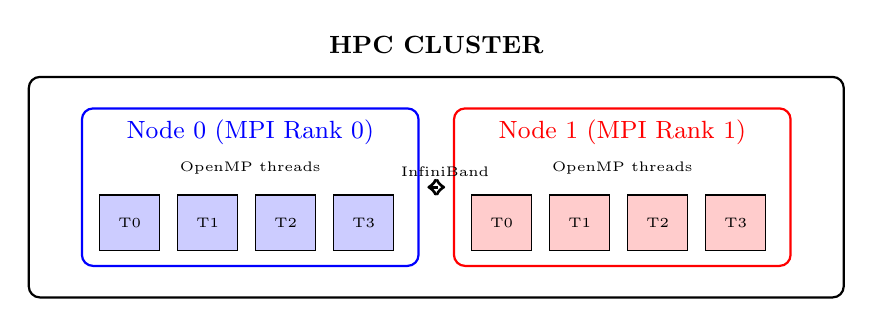
\begin{tikzpicture}[x=4.5cm,y=2cm]
    % Cluster box
    \draw[thick,rounded corners] (-0.15,-0.2) rectangle (2.15,1.2);
    \node[font=\small\bfseries] at (1,1.4) {HPC CLUSTER};

    % Node 0
    \draw[blue,thick,rounded corners] (0,0) rectangle (0.95,1);
    \node[font=\small,blue] at (0.475,0.85) {Node 0 (MPI Rank 0)};
    \foreach \t in {0,1,2,3} {
        \draw[fill=blue!20] (0.05+\t*0.22,0.1) rectangle (0.22+\t*0.22,0.45);
        \node[font=\tiny] at (0.135+\t*0.22,0.275) {T\t};
    }
    \node[font=\tiny] at (0.475,0.62) {OpenMP threads};

    % Node 1
    \draw[red,thick,rounded corners] (1.05,0) rectangle (2,1);
    \node[font=\small,red] at (1.525,0.85) {Node 1 (MPI Rank 1)};
    \foreach \t in {0,1,2,3} {
        \draw[fill=red!20] (1.1+\t*0.22,0.1) rectangle (1.27+\t*0.22,0.45);
        \node[font=\tiny] at (1.185+\t*0.22,0.275) {T\t};
    }
    \node[font=\tiny] at (1.525,0.62) {OpenMP threads};

    % Network arrow
    \draw[<->,very thick,dashed] (0.975,0.5) -- (1.025,0.5)
          node[above,font=\tiny]{InfiniBand};
\end{tikzpicture}
\end{center}

\subsection{The Problem with Pure MPI on a Cluster}

With $P$ nodes, each having $T$ cores:

\begin{itemize}
    \item \textbf{Pure MPI} ($P \times T$ processes): cores on the
          \emph{same} node communicate through MPI, even though they share
          RAM and could read each other's data directly.  This wastes network
          bandwidth and adds latency.
    \item \textbf{Pure OpenMP}: limited to one node — cannot cross node
          boundaries.
    \item \textbf{Hybrid}: MPI at the coarse level (between nodes), OpenMP at
          the fine level (within each node).  Best of both worlds.
\end{itemize}

\subsection{Two-Level Parallelism}

\begin{center}
\begin{tabular}{lll}
\toprule
Level & Technology & Grain \\
\midrule
Coarse & MPI & Different ranks own different user rows \\
Fine & OpenMP & Threads within a rank share work over its rows \\
\bottomrule
\end{tabular}
\end{center}

With $P$ MPI processes and $T$ threads each:
\[
\text{Total workers} = P \times T
\]

But the MPI communication is only between $P$ processes (not $P \times T$),
reducing message count and network load.

% =============================================================================
\section{MPI Thread Safety: \texttt{MPI\_Init\_thread}}
% =============================================================================

When threads exist inside an MPI rank, MPI must know about it.  Use
\texttt{MPI\_Init\_thread} instead of \texttt{MPI\_Init}:

\begin{lstlisting}
int provided;
MPI_Init_thread(&argc, &argv, MPI_THREAD_FUNNELED, &provided);
if (provided < MPI_THREAD_FUNNELED)
    fprintf(stderr, "Warning: MPI thread support below FUNNELED.\n");
\end{lstlisting}

\subsection{Thread Safety Levels}

MPI defines four levels of thread safety, in increasing capability:

\begin{center}
\begin{tabular}{lp{8cm}}
\toprule
Level & Meaning \\
\midrule
\texttt{MPI\_THREAD\_SINGLE} &
  Only one thread will execute (no OpenMP; pure MPI). \\
\texttt{MPI\_THREAD\_FUNNELED} &
  Multiple threads exist, but only the \emph{main thread} calls MPI.
  (Our case: MPI collectives are called outside parallel regions.) \\
\texttt{MPI\_THREAD\_SERIALIZED} &
  Any thread may call MPI, but not simultaneously (app must serialise). \\
\texttt{MPI\_THREAD\_MULTIPLE} &
  Any thread may call MPI at any time (most flexible, most overhead). \\
\bottomrule
\end{tabular}
\end{center}

\textbf{Why \texttt{FUNNELED} for our program?}  We call
\texttt{MPI\_Allgatherv} and \texttt{MPI\_Reduce} only from the main thread
(outside \texttt{\#pragma omp parallel} blocks).  Inside parallel regions,
threads never call MPI — they only work on local data.  This satisfies
\texttt{MPI\_THREAD\_FUNNELED} and allows MPI implementations to skip the
overhead of higher safety levels.

% =============================================================================
\section{Two-Level Parallelism in Each Phase}
% =============================================================================

\subsection{Phase 2: User Means}

\begin{lstlisting}
/* Level 1 (MPI): rank r is responsible for users [start_u, end_u) */
/* Level 2 (OpenMP): threads within rank divide [start_u, end_u) */

#pragma omp parallel for schedule(static)
for (int u = start_u; u < end_u; u++) {
    double sum = 0.0; int cnt = 0;
    for (int i = 0; i < N_ITEMS; i++)
        if (R(u, i) != 0.0f) { sum += R(u, i); cnt++; }
    user_mean[u] = (cnt > 0) ? (float)(sum / cnt) : 3.0f;
}
/* OpenMP implicit barrier: all threads done before MPI call */

/* Level 1 (MPI): share all slices */
MPI_Allgatherv(&user_mean[start_u], end_u - start_u, MPI_FLOAT,
               user_mean, recvcounts, displs, MPI_FLOAT, MPI_COMM_WORLD);
\end{lstlisting}

\textbf{Critical ordering:}  The OpenMP implicit barrier at the end of
\texttt{\#pragma omp parallel for} ensures \emph{all} threads have finished
writing \texttt{user\_mean[]} before the main thread calls
\texttt{MPI\_Allgatherv}.  This satisfies \texttt{MPI\_THREAD\_FUNNELED}.

\subsection{Phase 3: Similarity Matrix}

\begin{lstlisting}
/* Level 2 (OpenMP): threads split the rank's rows dynamically */
#pragma omp parallel for schedule(dynamic, 4)
for (int u = start_u; u < end_u; u++) {
    SIM(u, u) = 1.0f;
    for (int v = 0; v < N_USERS; v++) {
        if (v == u) continue;
        SIM(u, v) = pearson_similarity(u, v);
    }
}
/* OpenMP barrier here */

/* Level 1 (MPI): assemble full sim_matrix on all ranks */
MPI_Allgatherv(&sim_matrix[start_u * N_USERS],
               (end_u - start_u) * N_USERS, MPI_FLOAT,
               sim_matrix, recvcounts, displs, MPI_FLOAT,
               MPI_COMM_WORLD);
\end{lstlisting}

\textbf{Why \texttt{schedule(dynamic, 4)}?}  Even within a rank's row slice,
the amount of work per row can vary based on sparsity (number of co-rated
items affects \texttt{pearson\_similarity} inner loop count).  Dynamic
scheduling prevents thread starvation.

\subsection{Phase 4: Predictions (No MPI)}

\begin{lstlisting}
#pragma omp parallel
{
    /* Thread-private nbrs buffer -- each thread allocates its own */
    SimPair *nbrs = (SimPair *)malloc(N_USERS * sizeof(SimPair));

    #pragma omp for schedule(dynamic, 2)
    for (int u = start_u; u < end_u; u++) {
        /* ... prediction logic ... */
    }
    free(nbrs);
}
/* No MPI needed: sim_matrix is complete on every rank from Phase 3 */
\end{lstlisting}

Phase 4 is the most computation-intensive phase where both levels give full
benefit: MPI partitions the users, OpenMP threads within each rank divide
that partition further.

\subsection{Phase 5: Two-Level Reduction}

\begin{lstlisting}
double local_err = 0.0; int local_cnt = 0;

/* Level 2 (OpenMP): threads accumulate partial sums */
#pragma omp parallel for reduction(+:local_err, local_cnt) schedule(static)
for (int t = 0; t < test_size; t++) {
    int u = test_set[t].user;
    if (u < start_u || u >= end_u) continue;
    local_err += fabs(PRED(u, test_set[t].item) - test_set[t].rating);
    local_cnt++;
}
/* OpenMP combines private copies into local_err, local_cnt */

double global_err = 0.0; int global_cnt = 0;

/* Level 1 (MPI): sum across all ranks to rank 0 */
MPI_Reduce(&local_err, &global_err, 1, MPI_DOUBLE, MPI_SUM, 0, MPI_COMM_WORLD);
MPI_Reduce(&local_cnt, &global_cnt, 1, MPI_INT,    MPI_SUM, 0, MPI_COMM_WORLD);

if (mpi_rank == 0)
    printf("[Eval] MAE = %.4f\n", (float)(global_err / global_cnt));
\end{lstlisting}

The reduction mirrors the two-tier parallelism:
\begin{enumerate}
    \item \textbf{OpenMP reduction}: private copies per thread, merged at barrier
    \item \textbf{MPI\_Reduce}: per-rank totals summed to rank 0
\end{enumerate}

% =============================================================================
\section{Configurations Benchmarked}
% =============================================================================

\begin{center}
\begin{tabular}{llll}
\toprule
Configuration & MPI processes & OMP threads & Total workers \\
\midrule
Hybrid\_2x4 & 2 & 4 & 8 \\
Hybrid\_4x2 & 4 & 2 & 8 \\
Hybrid\_8x1 & 8 & 1 & 8 (effectively pure MPI) \\
Hybrid\_1x8 & 1 & 8 & 8 (effectively pure OpenMP) \\
\bottomrule
\end{tabular}
\end{center}

Comparing these reveals the communication overhead of MPI vs.\ the thread
overhead of OpenMP for the same total worker count.

% =============================================================================
\section{Why Hybrid Outperforms Pure MPI on a Single Node}
% =============================================================================

On a single machine, all processes share the same physical memory even in MPI.
However, MPI still treats them as separate address spaces and routes data
through system buffers.  OpenMP threads truly share memory — no copying.

\textbf{Scenario:} 8-core machine, similarity phase
\begin{center}
\begin{tabular}{lll}
\toprule
Approach & Communication & Overhead source \\
\midrule
Pure MPI (8 proc.) & 8-way Allgatherv through buffers & Memory copy overhead \\
Pure OpenMP (8 thr.) & No communication & Cache coherence only \\
Hybrid 2$\times$4 & 2-way Allgatherv & Minimal; threads share within node \\
\bottomrule
\end{tabular}
\end{center}

On a multi-node cluster, the hybrid gives the best of both:
\begin{itemize}
    \item MPI handles \emph{inter-node} data transfer (unavoidable)
    \item OpenMP handles \emph{intra-node} parallelism (zero copy overhead)
    \item Total MPI messages = $P$ (not $P \times T$)
\end{itemize}

% =============================================================================
\section{Compile and Run}
% =============================================================================

\begin{verbatim}
# Compile (mpicc + -fopenmp enables both MPI and OpenMP)
mpicc -O2 -Wall -fopenmp -o hybrid_rec hybrid/hybrid_recommender.c -lm

# Run configurations (total workers = P x T):
mpirun -np 2 env OMP_NUM_THREADS=4 ./hybrid_rec 1000 1000  # 2x4=8
mpirun -np 4 env OMP_NUM_THREADS=2 ./hybrid_rec 1000 1000  # 4x2=8
mpirun -np 8 env OMP_NUM_THREADS=1 ./hybrid_rec 1000 1000  # 8x1=8
mpirun -np 1 env OMP_NUM_THREADS=8 ./hybrid_rec 1000 1000  # 1x8=8
\end{verbatim}

\textbf{Note on \texttt{env}:}  The \texttt{env OMP\_NUM\_THREADS=4}
prefix sets the environment variable for the launched processes.  This is
more portable than \texttt{export OMP\_NUM\_THREADS=4} before \texttt{mpirun}.

% =============================================================================
\section{Differences from Pure MPI and Pure OpenMP}
% =============================================================================

\begin{center}
\begin{tabular}{lll}
\toprule
Feature & MPI only & Hybrid \\
\midrule
Include & \texttt{<mpi.h>} & \texttt{<mpi.h>} + \texttt{<omp.h>} \\
Init & \texttt{MPI\_Init} & \texttt{MPI\_Init\_thread(FUNNELED)} \\
Workers & $P$ processes & $P$ processes $\times$ $T$ threads each \\
Similarity kernel & Serial per rank & OpenMP parallel inside each rank \\
Messages & $P$-way Allgatherv & $P$-way Allgatherv (same!) \\
MAE reduction & MPI\_Reduce & OpenMP reduction $+$ MPI\_Reduce \\
Compile & \texttt{mpicc} & \texttt{mpicc -fopenmp} \\
\bottomrule
\end{tabular}
\end{center}

% =============================================================================
\section{Key Points to Explain in a Presentation}
% =============================================================================

\begin{enumerate}
    \item \textbf{What is two-level parallelism?}  MPI divides work at the
          coarse grain (between nodes/processes), OpenMP divides it at the fine
          grain (between threads within a process sharing memory).  The result
          is $P \times T$ effective workers with only $P$ MPI messages.
    \item \textbf{Why is \texttt{MPI\_Init\_thread} necessary?}  When threads
          exist inside an MPI process, MPI needs to know so it can guarantee
          thread safety.  \texttt{FUNNELED} means only the main thread calls
          MPI, which is exactly what our code does.
    \item \textbf{Why do MPI calls happen only outside OpenMP parallel regions?}
          Because we requested \texttt{MPI\_THREAD\_FUNNELED}.  If a worker
          thread inside a \texttt{\#pragma omp parallel} block called
          \texttt{MPI\_Allgatherv}, it would violate this contract and produce
          undefined behaviour (possibly a crash or deadlock).
    \item \textbf{How does the two-level reduction work?}  OpenMP's
          \texttt{reduction(+:local\_err)} merges per-thread partial sums within
          each rank.  Then \texttt{MPI\_Reduce} merges the per-rank totals.
          Total additions: $T-1$ (OpenMP) $+ P-1$ (MPI) = $P+T-2$ instead
          of $P \times T - 1$ serial additions.
    \item \textbf{What configuration should you choose on a real cluster?}
          Set MPI processes = number of nodes; set OpenMP threads = cores per
          node.  This eliminates all intra-node MPI traffic and maximises
          the benefit of shared memory within each node.
\end{enumerate}

\vfill
\begin{center}
    \small\textit{Group 11 — EC7207 High Performance Computing}
\end{center}

\end{document}
